% Direction-of-arrival diagram
% Author: Edgar Fuentes
\documentclass{article}
\usepackage{tikz}
\usetikzlibrary{shapes.geometric}
\usetikzlibrary{shapes.arrows}
\usepackage{array}
\begin{document}
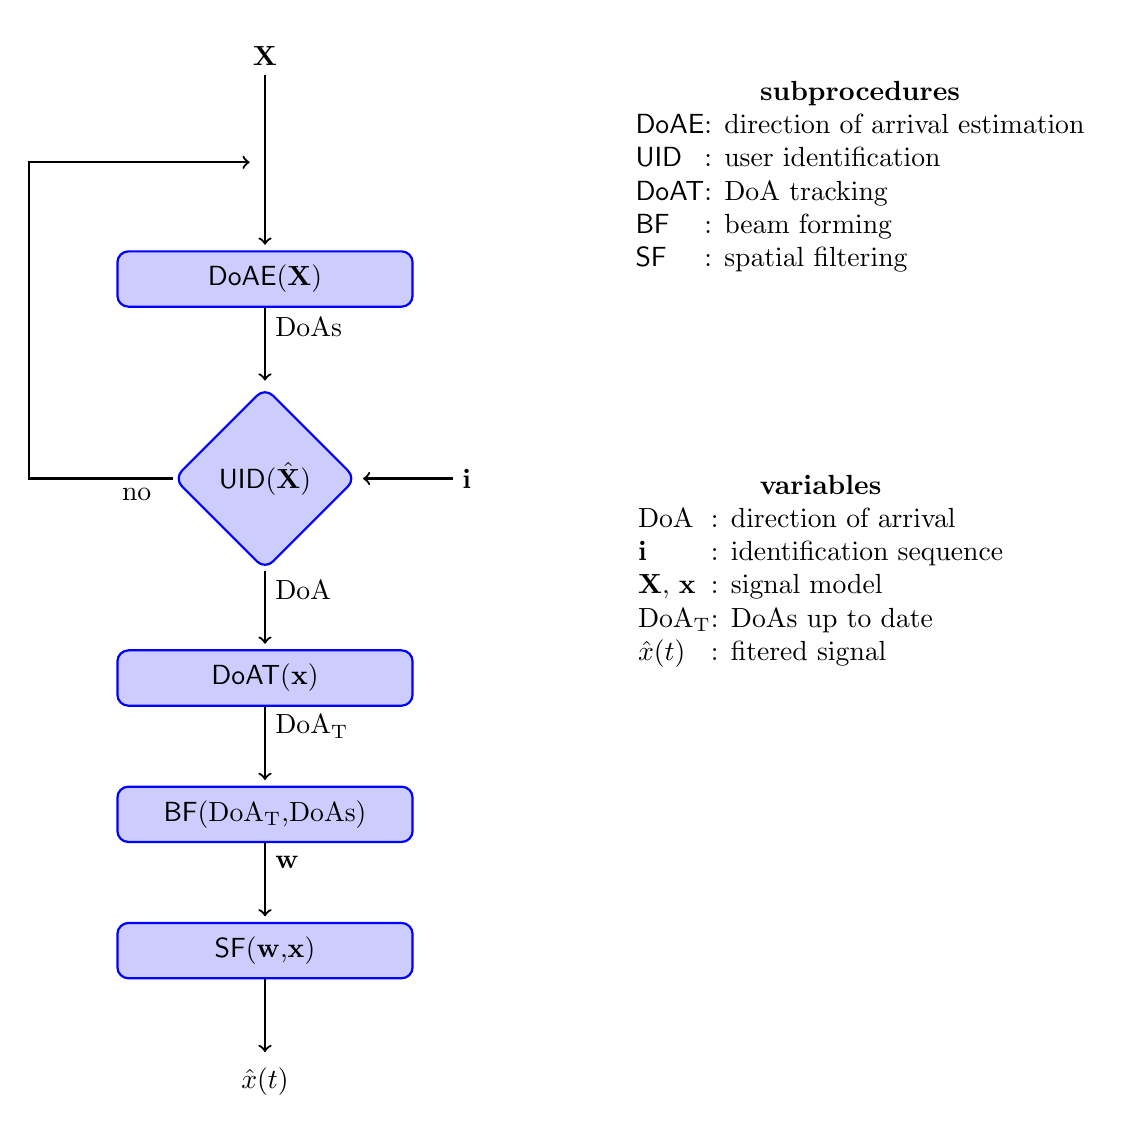
\begin{tikzpicture} [
    auto,
    decision/.style = { diamond, draw=blue, thick, fill=blue!20,
                        text width=5em, text badly centered,
                        inner sep=1pt, rounded corners },
    block/.style    = { rectangle, draw=blue, thick, 
                        fill=blue!20, text width=10em, text centered,
                        rounded corners, minimum height=2em },
    line/.style     = { draw, thick, ->, shorten >=2pt },
  ]
  % Define nodes in a matrix
  \matrix [column sep=5mm, row sep=10mm] {
                    & \node [text centered] (x) {$\mathbf{X}$};            & \\
                    & \node (null1) {};                                    & \\
                    & \node [block] (doa) {\textsf{DoAE}($\mathbf{X}$)};   & \\
    \node(null3){}; & \node [decision] (uiddes)
                        {\textsf{UID}($\hat{\mathbf{X}}$)};
                                  & \node[text centered](tra){$\mathbf{i}$}; \\
                    & \node [block] (track) {\textsf{DoAT}($\mathbf{x}$)}; & \\
                    & \node [block] (pesos)
                        {\textsf{BF}(DoA$_{\mathrm{T}}$,DoAs)};            & \\
                    & \node [block] (filtrado)
                        {\textsf{SF}($\mathbf{w}$,$\mathbf{x}$)};          & \\
                    & \node [text centered] (xf) {$\hat{x}(t)$ };          & \\
  };
  % connect all nodes defined above
  \begin{scope} [every path/.style=line]
    \path (x)        --    (doa);
    \path (doa)      --    node [near start] {DoAs} (uiddes);
    \path (tra)      --    (uiddes);
    \path (uiddes)   --++  (-3,0) node [near start] {no} |- (null1);
    \path (uiddes)   --    node [near start] {DoA} (track);
    \path (track)    --    node [near start] {DoA$_{\mathrm{T}}$} (pesos);
    \path (pesos)    --    node [near start] {\textbf{w}} (filtrado);
    \path (filtrado) --    (xf);
  \end{scope}
  %
  % legend for subprocedures
  \node (leyend) at (7.5, 5){
    \begin{tabular}{>{\sffamily}l@{: }l}
      \multicolumn{2}{c}{\textbf{subprocedures}} \\
      DoAE & direction of arrival estimation     \\
      UID  & user identification                 \\
      DoAT & DoA tracking                        \\
      BF   & beam forming                        \\
      SF   & spatial filtering
    \end{tabular}
  };
  %
  % legend for input and output variables
  \node (leyend) at (7, 0){
    \begin{tabular}{l@{: }l}
      \multicolumn{2}{c}{\textbf{variables}}              \\
      DoA                       & direction of arrival    \\
      $\mathbf{i}$              & identification sequence \\
      $\mathbf{X},\,\mathbf{x}$ & signal model            \\
      DoA$_{\mathrm{T}}$        & DoAs up to date         \\
      $\hat{x}(t)$              & fitered signal
      \end{tabular}
  };
\end{tikzpicture}
\end{document}